\chapter{Modelling microstructure noise}
\label{chap:modelling_microstructure_noise}
\section{Introduction}
When modeling financial transaction data, particular attention is given to certain distinctive properties of such data, one of which is the irregular spacing in time between events. This characteristic leads to the modeling of financial time series as a point process, specifically referred to as a financial point process. In this context, the inter-event waiting times are classified into three categories:
\begin{itemize}
	\item \textbf{Trade/Quote Duration Time}: This represents the time between two consecutive trade or quote arrivals.
	
	\item \textbf{Price Duration Time}: It measures the time it takes for cumulative absolute price changes of a given magnitude to occur.
	
	\item \textbf{Volume Duration Time}: This denotes the time it takes until a cumulative order volume of a specified size is traded.
\end{itemize}
By analyzing these inter-event waiting times and their characteristics, we can gain valuable insights into the dynamics of financial markets and develop models to better understand and predict market behavior.\\
From empirical data, Poissonian distribution does not fit inter-arrival trade times:
\begin{center}
	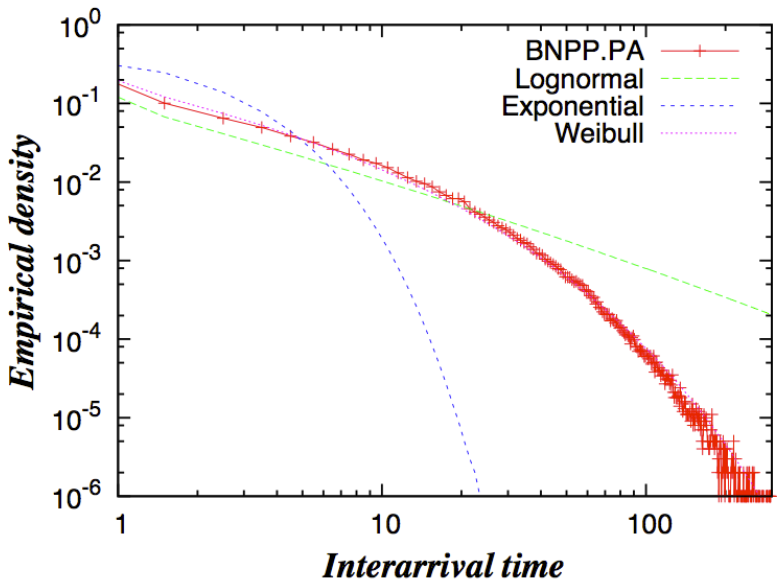
\includegraphics[width=0.5\textwidth]{picture/(39)interarrival_trade_times.png}
\end{center}
And analysing ACF, we notices a strong positive correlation, exists a memory.
\begin{mydefinition}[Point process]
A financial point process is a simple temporal marked point process, characterized by:
\begin{itemize}
	\item $\{t_i\}_{i \in \{1,\ldots,n\}}$: random sequence of increasing event times, $0:=t_0<t_2<\ldots<t_n$
	\item $N:$ cadlag counting process, $N_t := \sum_{1\geq 1} \mathds{1}_{\{t_i \leq t\}}$ s.t. $\expected{N_t} < \infty, \quad \forall t \geq 0$
	\item $x_i:= t_i - t_{i-1}, i=1,\ldots,n:$inter-event durations
	\item $x$: backward recurrence time, defined by $x(t):= t - t_{\breve{N}_t}$, where ${\breve{N}_t}:= \sum_{i \geq 1} \mathds{1}_{\{t_i < t\}}$ 
	\item $\mathcal{F}^N$: internal history of the point process
	\item  $\mathcal{F}_t$: a more general filtration including covariates $\mathcal{F}_t^N \subseteq\mathcal{F}_t$
\end{itemize}
\end{mydefinition}
A counting process $N_t$ is a submatringale,since:
\[
\expected{N_t| \{N_\tau: \tau \leq s\}}\geq N_s \qquad \forall s \leq t
\]
\begin{mydefinition}[Compensator]
According to Doob-Meyer decomposition there is a unique predictable increasing process such that $\Lambda_0=0$, $\Lambda_\infty$ is integrable, and $N_t = M_t + \Lambda_t$  with $M$ an uniformly
integrable $\mathcal{F}$-martingale. $\Lambda$ is a $\mathcal{F}-$compensator of $N$.
\end{mydefinition}
In a Poisson process with rate $\lambda$, the compensator is $\Lambda_t = \lambda t$, since:
\[
\expected{N_t - \lambda t| \{N\tau: \tau \leq s\}} = 0
\] 
$N_t - \lambda t$ is an $\mathcal{F}-$ martingale
\begin{mydefinition}[Intensity function]
The $\mathcal{F}$-intensity function $\lambda_t$ of $N$ is a scalar positive $\mathcal{F}-$predictable process defined by:
\[
\Lambda_t = \int_0^t \lambda_udu
\]
It can also be defined by:
\[
\expected{N_t - N_s|\mathcal{F}} = \expected{\int_s^t \lambda_udu| \mathcal{F}_s} \qquad \forall 0\leq s \leq t
\]
so:
\[
\lambda_{t+} := \lim_{\Delta \to 0^+} \lambda_{t + \Delta} = \lim_{\Delta \to 0^+} \frac{1}{\Delta} \expected{N_{t +\Delta} - N_t| \mathcal{F}_t}
\]
we define the probability in unite per time to observe a count
\end{mydefinition}
\begin{mydefinition}[Survivor function]
Let $X$ be the random variable describing the inter-event durations; $f(x)$ is its probability density function and $S(x)$ the survivor function:
\[
S(x) := 1 - F(x) = 1 - Pr[X \geq x] = Pr[X>x]
\]
\end{mydefinition}
\begin{mydefinition}[Hazard function]
The Hazard function $h(x)$ off a point process is defined as
\[
h(x):= \frac{f(x)}{S(x)} = \lim_{\Delta \to 0} \frac{1}{\Delta}Pr[x\leq X < x + \Delta| X \geq x]
\]
\end{mydefinition}
A point process can be equivalently defined by three differnet representation: intensity, duration and counting representation:
\begin{mydefinition}[Intensity representation]
\begin{align*}
	& Pr[(N_{t + \Delta} -N_t)=1|\mathcal{F}_t]=\lambda \Delta + o(\Delta)\\
	& Pr[(N_{t + \Delta} -N_t)>1|\mathcal{F}_t]= o(\Delta)
\end{align*}
where $\lambda >0$ is the constant Poisson rate
\end{mydefinition}

\begin{mydefinition}[Duration representation]
\[
x_i \sim i.i.d(\text{Exp}(\lambda))
\]
\end{mydefinition}
\begin{mydefinition}[Counting representation]
Let $N_{(a,b])} := N_b - N_a$ then:
\[
Pr[N_{(a,b])} = k] = e^{-\lambda(b-s)}\frac{(\lambda (b-a))^k}{k!}
\]
\end{mydefinition}
Let make an example for a non-homogeneous Poisson process:
\begin{itemize}
    \item \textbf{intensity representation}:
    \begin{align*}
    	& Pr[(N_{t + \Delta} -N_t)=1|\mathcal{F}_t]=\lambda_t \Delta + o(\Delta)\\
    	& Pr[(N_{t + \Delta} -N_t)>1|\mathcal{F}_t]= o(\Delta)
    \end{align*}
    where $\lambda_t >0$ is the intensity function
    \item \textbf{duration representation}: $x_i \sim i.i.d(\text{Exp}(\Lambda_{t_i +1} - \Lambda_{t_i}))$
    \item \textbf{counting representation}: let $\Lambda(a,b):= \lambda_d - \Lambda_a = \int_a^b \lambda_sds$,:
    \[
    Pr[N_{(a,b]} = k] - e^{-\Lambda(a,b)} \frac{(\Lambda(a,b))^k}{k!}
    \] 
\end{itemize}
\begin{mydefinition}[Multivariate point process]
A $K-$variate point process is a process $\{t_i,d_i\}_{i\in (1,\ldots,n)}$ on $(0,\infty)$, where:
\begin{itemize}
	\item $d_i \in \{1,\ldots,K\}$ is a random variable representing $K$ different types of events
	\item $\{t_i^k\}_{i\in \{1,\ldots,n^k\}}, k =1,\ldots,K$ are the arrival times
	\item $N_t^k = \sum_{i\geq 1} \mathds{1}_{\{t_i \leq t\}} \mathds{1}_{\{d_i = k\}}$
\end{itemize}
\end{mydefinition}
\newpage
\begin{mytheorem}[Random Time Change Theorem]
	Given a $K$-varaite point process $N  = (N^1,\ldots, N^k)$ with event times $\{t_i^k\}_{i\in \{1,\ldots,n^k\}}$, $k=1,\ldots,K$ and compensators $\Lambda = (\Lambda^1,\ldots, \Lambda^k)$ s.t $\Lambda^k_\infty = \infty, \forall k = 1,\ldots,K.$ Then the $K$ scalat point processes with event times $\{\Lambda^k_{t_i^k}\}_{i \in \{1,\ldots, n^k\}}, k=1,\ldots,K$ are independent homogeneoud Poisson processes with unit intensity.
\end{mytheorem}
The random time change theorem plays an important role in order to construct diagnostic tests for point process models or to simulate point processes, in fact: we estimate with $\Lambda_t$, using theorem we obtain $\Lambda$ from $\lambda$, I plot a qqplot and evaluate if process is poisson process.\\
\section{Model}
Models of the discrete time duration process $\{x_i\}_{i=1,\ldots,n}$ observable at the event times $\{t_i\}_{i=1,\ldots,n}$ obtained parametrizing either the conditional distribution function $F(x_i|\mathcal{F}_{t_{i-1}})$ or the hazard rate $h(x_i|\mathcal{F}_{t_{i-1}}$
)
\begin{mytheorem}[Proportional Hazard model (Cox 1972)]
	\[h(x|z;\theta) = h_0(x|\gamma_1)g(z,\gamma_2)\]
where $\theta = (\gamma_1,\gamma_2)$ is the baselime hazard rate and $g$ is a function of covariates $z$ and parameters $\gamma_2$
\end{mytheorem}
The baseline hazard rate $h_0$ can be parametrized by a Weibull distribution with parameters $\lambda$ and $p$
\[
h_0(x|\gamma_1) = \lambda(\lambda x)^{p-1}
\]
which is the hazard rate associated with the pdf:
\[
f(x) = \begin{cases}
	\lambda p(\lambda x)^{p-1} e^{- (\lambda x)^p} & x\geq 0\\
	0 & x<0
\end{cases}
\]
we can distinguish three cases:
\begin{itemize}
	\item $p=1 \to h_0(x|\gamma_1) = \lambda$ (exponential, no memory, it is not dependent on $x$)
	\item $p>1 \to \partial_x h_0(x|\gamma_1) >0$ (positive duration dependence)
	\item $p<1 \to \partial_x h_0 (x|\gamma_1) <0$ (negative duration dependence)
\end{itemize}
\subsection{Autoregressive Conditional Duration}
Let us denote by $x_i:= \frac{t_i - t_{i-1}}{s(t_i)}$ the inter-event duration normalized by a seasonality factor $s(t_i)$.\\
Engle and Ruseel in 1997 proposed that $x_i = \Psi_i \epsilon_i$ where $\epsilon_i$ are i.i.d positive random variables with $\expected{\epsilon_i} =1$, so:
\[
\Psi_i = \expected{x_i| \mathcal{F}_{t_i-1}}
\]
is the conditional duration mean.\\
The model can be rewritten in the terms of the intenisty as:
\[
\lambda(t|\mathcal{F}_t) = \lambda_\epsilon \left(\frac{x(t)}{\Psi_{\breve{N}(t) + 1}}\right) \frac{1}{\Psi_{\breve{N}(t) +1}}
\]
where $\lambda_\epsilon(s)$ is the hazard function of the errore term 
\begin{mytheorem}[Exponential ACD model (Dufour and Engle 2000)]
	\[
	\epsilon_i \sim i.i.d(Exp(1)) \qquad \to \qquad \lambda(t|\mathcal{F}_t) = \frac{1}{\Psi_{\breve{N}_{t+1}}}
    \]
Typically $\Psi_i$ is choosen to be a function of the past information set $\mathcal{F}_{t_i-1}$ as \\ $\Psi_i = \Psi(\Psi_{i-1},\ldots, \Psi_{i-q}, x_{i-1},\ldots,x_{i-p})$
\end{mytheorem}
\begin{mytheorem}[Linear ACD model]
	The generic ACD(r,s) model is:
	\[
	\psi_i = \omega + \sum_{j=1}^{r} \alpha_jx_{i-j} + \sum_{j=1}^{s} \beta_j \Psi_{i-j}
	\]
\end{mytheorem}
Similar to GARCH models, the process $\eta_i =x_i -\Psi_i$ is a Martingale difference sequence $(\expected{\eta_i|\mathcal{F}_{i-1}}=0)$ and the ACD can be written as:
\[
x_i = \omega + \overbrace{\sum_{j=1}^{\max(r,s)} (\alpha_j + \beta_j)x_{i-j}}^{\text{autoregressive}} - \underbrace{\sum_{j=1}^{s} \beta_j \eta_{i-j} + \eta_j}_{\text{mean average}}
\]
This is an ARMA representation with non Gaussian innovations.\\ Taking expections of both sides od the last expression and assuming stationarity:
\[
\expected{x_i} = \frac{\omega}{1 - \sum_{j=1}^{\max(r,s)} (\alpha_j + \beta_j)}
\]
hence we need to assume that $\sum_{j=1}^{\max{(r,s)}} (\alpha_j + \beta_j) <1$.\\
\subsection{EACD(1,1) model}
\[
x_i = \Psi_i \epsilon_i \qquad \epsilon_i \sim i.i.d(Exp(1)) \qquad \Psi_i = \omega + \alpha_1 x_{i-1} + \beta_i \Psi_{i-1}
\]
Evaluating the expected value of each element, we obtain:
\[
\expected{\epsilon_i} =1 \qquad Var[\epsilon_i] =1 \qquad \expected{\epsilon_i^2} = 2
\]
We have:
\[
\expected{x_i} = \expected{\expected{\psi_i\epsilon_i| \mathcal{F}_{i-1}}} = \expected{\psi_i}  \qquad \expected{\psi_i}= \omega + \alpha_1\expected{x_{i-1}} + \beta_i \expected{\psi_{i-1}}
\]
under weak stationarity:
\[
\mu_x := \expected{x_i} = \expected{\psi_i} = \frac{\omega}{1 - \alpha_1 - \beta_1}
\]
Moreover $\expected{x_i^2} =\expected{\expected{\psi_i^2 \epsilon_i^2| \mathcal{F}_{i-1}}} = 2 \expected{\psi_i^2}$
With similar arguments we can show that:
\begin{align}
	&Var[x_i] = \mu^2_x \frac{1 - \beta_1^2 - 2 \alpha_1\beta_1}{1 - \beta_1^2 - 2\alpha_1 \beta_1 - 2 \alpha_1^2}\\
	&\rho_1 :=  Corr[x_i,x_{i-1}] = \frac{\alpha_1 (1 - \beta_1^2 - \alpha\beta)}{1 -\beta_1^2 - 2\alpha_1 \beta_1}\\
	&\rho_k := Corr[x_i, x_{i-k}] = (\alpha-1 + \beta_1) \rho_{k-1} \qquad \forall k\geq 2
\end{align}
From the first we can evaluate that the duration process is covariance stationary if:
\[
\beta_1^2 + 2\alpha_1 \beta_1 + 2\alpha_1^2 <1
\]
From the third we notice that ACF decreases at a geometric rate (while real data can also exhibit a hyperbolic ACF
)
\subsection{Estimation of ACD models}
For an ACD(r,s) model, setting $i_0 = \max(r,s)$, the likelihood of the durations, $x_1,\ldots,x_T$ is:
\[
f(\mathbf{x}_T| \theta) = \left[\prod_{i=i_0 +1}^{T} f(x_i|\mathcal{F}_{i-1},\theta)\right] \times f(\mathbf{x}_{i_0}|\theta)
\]
Conditional likelihood is much easier to handle and essentially equivalent for large $T$.\\
For a WACD the log-likelihood is:
\[
\ell(\mathbf{x}| \theta, \mathbf{x}_{i_0}) = \sum_{i = i_0 +1}^{T} p \ln \left[\Gamma \left(1 + \frac{1}{p}\right)\right] + \ln \left(\frac{p}{x_i}\right) + p \ln \left(\frac{x_i}{\Psi_i}\right) - \left[\frac{\Gamma\left(1 + \frac{1}{p}\right)x_i}{\Psi_i}\right]^p
\]
where $\Psi_i = \omega + \sum_{j=1}^r \alpha_j x_{i-j} + \sum_{j=1}^{s} \beta_j \psi_{i-j}$.\\
When $p=1$ we obtain the conditional log-likelihood for a EACD(r,s) model
\subsection{Logarithmic ACD model}
From ACD model is difficult to allow $\Psi_i$ to depend on functions of covariates without violating the non-negativity restriction. Bauwens and Giot (200) propose a class of logarithmic ACD models, where no parametric restriction are needed to ensure positiveness of the process:
\[
\ln \Psi_i = \omega + \beta_1 \ln \Psi_{i-1} + \alpha_1 g (\epsilon_{i-1}) \qquad \omega>0,\alpha,\beta\geq 0 
\]
\begin{align*}
	&\text{type }I \qquad g(\epsilon_{i-1}) = \ln \epsilon_{i-1}\\
	&\text{type }II \qquad  g(\epsilon_{i-1}) = \epsilon_{i-1}
\end{align*}
The duration process is covariance-stationary $iff$:
\[
\beta <1 \qquad \expected{\epsilon_i e^{\alpha g(\epsilon_i)}}<\infty \qquad \expected{e^{2\alpha g(\epsilon_i)}}<\infty
\]
\subsection{Autoregressive Conditional Intensity model (Russel, 1999)}
Let $\lambda(t) = (\lambda^1(t),\ldots, \lambda^K (t))'$, for $k=1,\ldots,K$:
\[
\lambda^k(t) = \Phi^k_{\breve{N}(t)+1} \lambda_0^k(t)s^k(t)
\]
where:
\begin{itemize}
	\item $\lambda_0^k$ is a baseline (determinstic) intensity
	\item $s^k(t)$ is a seasonali component
	\item $\Phi^k_i = \exp(\tilde{\Phi}^k_i + z'_{\tilde{t}_j} \gamma_k)$
	\item $z_i$ ate vectors of covariates observable at arrival time $t_i$ with parameter vector $\gamma^k$
\end{itemize}
The vector $\tilde{\Phi}_i = (\tilde{\Phi}_i^1,\ldots, \tilde{\Phi}_i^k)'$ is parametrized as:
\[
\tilde{\Phi}_i = \sum_{k=1}^{K} (A^k \epsilon_{i-1} + B^k \tilde{\Phi}_{i-1})y^k_{k-1}
\]
where $y_i^k = \mathds{1}_{\{t_i = t_j^*\}}$ and $A^k = (a_1^k,\ldots,a^k_K)'$ and $B^k = \{b_{ij}^k\}_{i,j =1,\ldots,K}$ and scalar innovation term $\epsilon_i$:
\[
\epsilon_i = \sum_{k=1}^K \left(1 - \int_{t^k_{N^k_{t_i}-1 }}^{t^k_{N^k_{t_i}}} \lambda^k(u) du\right)y_i^k
\]
The fundamental principle of the ACI model is that at each event occurrence at time $t_i$, all $K$ processes are updated based on the realization of the integrated intensity relative to the most recent process. Importantly, the impact of this innovation on the $K$ processes can vary, and it also depends on the type of the most recent point in the process sequence.
\subsection{Hawkes processes}
A different dynamic intensity model is obtained by specifying $\lambda(t)$ as a(linear) self-exciting process given by:
\[
\lambda(t) = \mu + \int_0^t \phi(t-s)dN(s) = \mu + \sum_{t_i <t} \phi(t-t_i)
\]
where $\phi(s)$ is a non-negative weight function and $\int_0^t \phi(s)dN(s)$ is the stochastic Stieltjes integral of the process $\phi$ with respect to the counting process $N(t)$
\begin{mytheorem}[Hawkes process]
	Hawkes process belong to the classs of mutually-exciting process, it is defined through its intensity function as:
	\[
	\lambda_i(t) = \mu_i + \sum_{j=1}^D \int_\infty^t \phi_{ij}(t-s)dN_j(s) = \mu_i + \sum_{i=1}^D \sum_{t_j<t} \phi_{ij}(t-t_j)
	\]
where:
\begin{itemize}
	\item $dN_j(s) = \sum_{t_j<s} \delta(s-t_j)ds$
	\item $\mu_i$ is a positive constant baseline intenisty
	\item the kernels $\phi_{ij}(t)$ are positive and causal functions in $L_1$
\end{itemize}
\end{mytheorem}
Denoting by $\mathbf{\Phi}(t)$ the kernel matrix:
\[
\mathbf{\Phi}(t) = \begin{pmatrix}
	\phi_{11}(t) & \ldots & \phi_{1D}(t) \\
	\vdots & \ddots & \vdots\\
	\phi_{D1}(t) & \ldots & \phi_{DD}(t)
\end{pmatrix}
\]
The process $N(t)$ has asymptotically statonary increments and $\lambda(t)$ is asymptotically stationary if the spectral radius of the matrix is:
\[
||\mathbf{\Phi}|| = \{||\phi_{ij}||\}<1 
\]
Utility of Hawkes processes:
\begin{itemize}
\item flexible and versatile tool to investigate mutual interaction (excitation); 
\item the linear structure of $\lambda(t)$ allows to compute many properties analytically; 
\item quantities have a clear interpretation;
\item availability of parametric and non-parametric estimation tools
\end{itemize}
\newpage
Hawkes processes, introduced more than four decades ago, have found significant utility in modeling earthquake data. In recent years, they have gained popularity in mathematical finance and econometrics, with various applications:
\begin{itemize}
\item Standard Applications: Hawkes processes are applied to model the arrival times of trades, buy-sell market orders, and mid-price changes in financial markets. These applications are found in research by Bowsher (2007) and Bauwens and Hautsch (2009).

\item Additional Examples: Other examples include modeling limit and market order flow in continuous double auction markets (Muni-Toke and Pomponio, 2012), studying the arrival of trades-through orders in a limit order book, and developing price impact models to replicate strong microscopic mean reversion and the Epps effect. Filimonov and Sornette (2012) introduced a measure based on Hawkes processes, aiming to provide insights into the level of endogeneity and its potential as a predictor of market micro-instabilities. However, Bouchaud and collaborators (2013) challenged this claim in a recent paper.

\item Contagion Modeling: Ait-Sahalia et al. (2012) propose a model for asset returns capable of capturing crisis periods characterized by contagion. In this model, the jump diffusion component of asset dynamics is described using a class of multi-dimensional Hawkes models. They discuss an estimation methodology based on the Generalized Method of Moments, although their analysis is limited to pairs of assets.

\item These applications demonstrate the versatility of Hawkes processes in modeling various aspects of financial markets and risk contagion.
\end{itemize}